

The goal of our fast path  is to forgo the overhead associated with two-phase transaction processing and communication with 
the TM to begin and commit transactions. This is particularly important for short transactions, where the begin and commit overhead is not amortized
across many operations.
We therefore focus on single-key transactions.

To this end, we introduce in Section~\ref{ssec:fast-api} a streamlined  \emph{fast path (FP)}
API that jointly executes multiple API calls of the original TPS, and 
%we refer to transactions that use this API as \emph{fast path (FP) transactions}. We 
define the semantics of FP transactions relative to regular ones.
% in Section~\ref{ssec:fast-semantics}.
We proceed, in Section~\ref{ssec:fast-algorithm}, to explain a high-level general fast path algorithm 
\inred{for any system that follows the generic schema of  Algorithm~\ref{alg:schema} above}. 
Finally, in Section~\ref{ssec:fast-impl}, we describe our implementation of the fast path in \sys, and 
important practical optimizations we did in this context.
 

 \remove{
   with SI semantics in the
context of a system following the generic schema of  Algorithm~\ref{alg:schema} above. 
Our solution consists of three parts: First, in Section~\ref{ssec:region-clock}, we enhance the
underlying data store with support for per-region \emph{Local Version Clocks (LVCs)}. 
This aspect is already implemented in CockroachDB, which uses 
per-region Hybrid Logical Clocks~\cite{Kulkarni2014LogicalPC} in order to allow for distributed timestamp allocation. 
In the systems that maintain a GVC, (e.g.,~\cite{Percolator2010,tephra,OmidICDE2014,omid-blog}), our 
addition of  LVCs 
entails a minor modification to management of global timestamps (in the transaction manager or oracle). 
Second, in Section~\ref{ssec:lvc-access}
we extend the underlying data store's API to allow manipulating 
a region's LVC jointly with objects stored at that region. 
Finally, we add client-side support for the fast path API, as explained in Section~\ref{ssec:lc-client}.
}

\subsection{API and semantics}
\label{ssec:fast-api}

\paragraph{API.}
For brevity, we refer to the TPS's API calls  begin, read, write, and commit as \code{b, r, w}, and \code{c} respectively, and 
we combine them to allow fast processing.
The basic FP transactions are singletons, i.e., transactions that perform a single
read or write. These are supported by the APIs: 
\begin{description}
\item[brc(key)] -- begins an FP transaction, reads key within it, and commits.
%Recall that read-only transactions don't need to commit. 
\item[bwc(key,val)] -- begins an FP transaction,  writes val into a new version of key that exceeds all existing ones, and commits.
\end{description}

We further support a fast path transaction consisting of a read and a dependent write, via a pair of API calls:
\begin{description}
\item[br(key)] -- begins an FP transaction and  reads the latest version of key. 
Returns the read value along with a \emph{handle} h for continuing the transaction.
\item[wc(h, key,val)] -- 	validates that key has not been written since the  \code{br} call that returned h, writes val into a new version of key, and commits.
\end{description}

Read-only transactions never abort, but \code{bwc} and \code{wc} may abort. 
If an FP transaction aborts, it can be retried either using the fast path again, or as a regular transaction.

\remove{
A more elaborate example is a read-modify-write API: 
\begin{description}
\item[brwc(key,f)] -- begins an FP transaction,  reads the latest version of key, applies $f$ to it (on the server side), 
	writes the result into a new version of key that exceeds all existing ones, and commits.
\end{description}

To use the above API, the programmer has to encapsulate the transaction logic in a function for server-side processing. 
Alternatively, we allow FP transactions to unfold dynamically much like regular  transactions do.
A dynamic FP transaction may instead begin with a \code{br} call, perform client-side processing, and then call the following
function to update either the same or a different key: 

\begin{description}
\item[wc(key,val)] -- writes val into a new version of key that exceeds all existing ones, and commits.
\end{description}

Moreover, we do not restrict FP transactions to perform a single read -- any number of \code{r}'s may be called between the \code{br} 
and \code{wc}. The supported types of FP transactions are summarized in Table~\ref{table:fp-types}.
Note, however, that all calls must be directed at the same region, else the transaction is not local.
In case an FP transaction dynamically discovers that it needs to access additional regions, it is aborted and should be restarted as a regular transaction. 

\begin{table}[htb]
%\def\arraystretch{1.5}%  1 is the default, change whatever you need
\centerline{
\begin{tabular}{l  @{\hspace{2em}} l}
Call sequence & Transaction type\\
\hline
\code{br} & single read\\
\code{bwc} & single write\\
\code{br, r*} &  multi-read\\
\code{br, r*, wc} & multi-read, single write\\
\code{brwc} & server-side single-read-write\\
%\hline
\end{tabular}
}
\caption{Supported FP transaction types.}
\label{table:fp-types}
\end{table}

In principle, it would have been possible to also allow \code{w} calls in the span of an FP transaction, 
but in this case, it is not possible to forgo the two-phase execution. 
That is, the \code{w} calls would need to indicate write intents, and  to be atomically committed (or aborted) during the final \code{wc} 
(or \code{c}) call. 
Given the limited benefit and extra complexity of allowing many writes in FP transactions, we do not support this option in our solution.

}

\paragraph{Semantics.}
%\label{ssec:fast-semantics}

The semantics for ordering FP transactions relative to regular ones are
weaker than SI in that they do not guarantee real-time order over all regular
and FP transactions together. For example, an FP transaction may return 
an older value than the latest one committed by a regular transaction. Similarly, a regular transaction overlapping
two FP ones may observe an update of the second and miss an update by the first,  as illustrated in Figure~\ref{fig:ltx-rt}.
However, we continue to enforce real-time order on regular transactions as well as on all updates of the same key.

\begin{figure}[h]
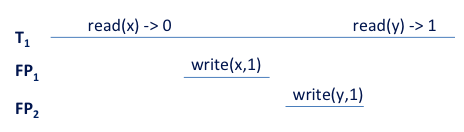
\includegraphics[width=\columnwidth]{figs/FP-semantics}
\caption{Possible violation of real-time order among fast path (FP) transactions. Regular transaction $T_1$
reads $x$ before it is updated by FP transaction $FP_1$ and reads $y$ after it is updated by FP transaction $FP_2$ even 
though $FP_2$ occurs after $FP_1$. 
%$T1$'s global version is $10$, and its skips the local version clocks of the regions holding $x$ and $y$ to $10$ when reading from them.
}
\label{fig:ltx-rt}
\end{figure}

Formally, the system enforces a total order ${\cal T}$ on all committed transactions, so that
\begin{enumerate}
    \setlength{\itemsep}{0pt}
    \setlength{\parskip}{0pt}
    \setlength{\parsep}{2pt}  
\item
regular transactions (though not FP ones) are ordered in ${\cal T}$  according to their commit times;
\item
non-overlapping transactions (regular and FP) that update the same key are ordered in ${\cal T}$  according to their commit times;
\item
each regular transaction's read operations see a consistent snapshot of the database reflecting 
a prefix of  ${\cal T}$ that includes  all transactions committed prior to
its start time; and 
\item
 a transaction commits only if none of the items it updates has been modified since that snapshot.
 \end{enumerate}

Note that  ${\cal T}$  preserves causality because 
only transactions that  access different data objects can be re-ordered.


\subsection{Generic fast path algorithm}
\label{ssec:fast-algorithm}



\begin{algorithm}[htb]
%\algblock[atomically do]{atomically}{EndAtomic}
\algblockdefx[atomic]{Atomic}{EndAtomic}
[0]{{\bf atomically do}}
[0]{}
%%%%%%%%
\begin{algorithmic}
\small
%\State local  \code{ts$_r$} \Comment  read version of ongoing transaction
%\Statex
\Procedure{brc}{key}
\State rec  $\leftarrow$ ds.get(last committed record of key) 
\State  return rec.value
\EndProcedure
%
\Statex
\Procedure{bwc}{key, value} 
	\State old $\leftarrow$ ds.get(last version of key)
	\If{old = nil}  \Comment found tentative value -- abort 
		\State return abort 
	\EndIf
	\State return {\sc writeVersion}(old, key, value)
\EndProcedure
%
\Statex
\Procedure{writeVersion}{old, key, value} 
	\State maxVersion $\leftarrow$ key's  maxVersion
	\State ver $\leftarrow$ $\max$(old, maxVersion) 
	\If{mask(ver, $2^\ell-1$) = $2^\ell-1$} 
		\State \Comment cannot increment version locally -- abort
		\State return abort 
	\EndIf
	\State 	ver $\leftarrow$ ver  $+1$ 
\Atomic 
	\If{ds.get(last version of key)  = old  }
	\State ds.put(\tuple{key, ver} with commit = ver)  
	\State {\sc bumpVersion}(key, ver)
	\State return commit
	\Else \State return abort \EndIf
\EndAtomic
\EndProcedure
%\Statex
\Procedure{bumpVersion}{key, $ts$} 
\Statex \Comment called by transactional read of key with  $ts_r = ts$
	\State {\bf atomically} set key's maxVersion to
	\State \hspace{10mm} $\max$($ts$, key's maxVersion) 
\EndProcedure
\Statex
\Procedure{br}{key} 
\State rec  $\leftarrow$ ds.get(last committed record of key) 
\State  return \tuple{rec.version, rec.value}
\EndProcedure
\Statex
\Procedure{wc}{h, key, value} 
\State return {\sc writeVersion}(h, key, value)
\EndProcedure

\end{algorithmic}
\caption{Generic support for FP transactions.}
\label{alg:fp}
\end{algorithm}

The generic fast fast path algorithm is given in Algorithm~\ref{alg:fp}. 
%
Singleton reads simply return the value associated wtih the  latest committed version of the requested key they encounter.  
They ignore tentative versions, which may lead to missing the latest commit in case its post-commit did not complete, 
but is allowed by our semantics. 
FP reads can forgo the begin call since they do not need to obtain a snapshot time a priori. 
They can also forgo the commit call, since they perform a single read, and hence their `snapshot' is trivially valid.

In case  \code{bwc} encounters a tentative version it does not try to resolve it, but rather simply aborts.
This may cause false aborts in case the transaction that wrote the tentative version has committed and did not 
complete post-commit. In other cases, it prioritizes regular transactions over FP ones. We choose this approach since
the goal is to complete FP transactions quickly, and if an FP transaction cannot complete quickly, it might as well be 
retried as a regular one.
   
A singleton write has two additional concerns: (1) it needs to  produce a new version number that exceeds all committed ones and
is smaller than any commit timestamp that will be assigned to a regular transaction in the future.
(2)  It needs to make sure that conflicts with regular transactions are detected. 

To support (1), we change the structure of timestamps to consist of two 
components -- a global version and a locally advancing sequence number.
Practically, we implement the two components in one long integer, with some number $\ell$ of the less significant bits
reserved to sequence numbers assigned by FP writes, and the the most significant bits representing 
the global version determined by the TM. Thus, the TM always produces timestamps where the $\ell$ lower bits are zeros,
and increases the global clock by $2^\ell$ on every begin and commit call.  

Singleton writes then read the object's latest committed version and increment it, provided that they can do so 
 without overflowing the sequence number. 
In case the lower $\ell$ bits are all ones, there is a need to increment the global clock, and so the FP transaction aborts and is retried
as a regular one. 

It is important to note that the singleton write needs to \emph{atomically} find the latest version and produce a new one that exceeds it, 
to make sure that no other transaction creates a newer version in the interim.
Below, we explain how we implement such atomic conditional updates in HBase as part of \sys. 

Next, we address (2), namely conflicts between FP and regular transactions.
Note that the atomic conditional write in \code{bwc} takes care of conflicts among singletons.
In case an ongoing regular transaction writes to a key before \code{bwc} accesses it, 
\code{bwc} finds the tentative write and aborts. It therefore remains to consider the case that
a regular transaction $T_1$ writes to some key after FP transaction $FP_1$, but must abort because 
it reads the old version of the key before $FP_1$'s update. This scenario is illustrated in Figure~\ref{fig:why-bump}. 

\begin{figure}[htb]
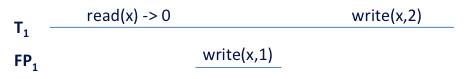
\includegraphics[width=\columnwidth]{figs/FP-why-bump}
\caption{Conflict between FP transaction $FP_1$ and regular transaction $T_1$.}
\label{fig:why-bump}
\end{figure}

In order for $T_1$ to detect this 
conflict, the version written by $FP_1$ has to exceed $T_1$'s snapshot time, i.e., $ts_r$.
To this end, we maintain a new field \emph{maxVersion} for each key, which is at least as 
high as the key's latest version. In addition, every transactional read \emph{bumps} key's version 
number to the reading transaction's $ts_r$. 
Writes consult this field and always select a new version that exceeds this value.
Thus, once $T_1$ reads key and bumps its \emph{maxVersion}, 
no FP transaction can write a version of key that should be 
included in $T_1$'s snapshot.

The  \code{br} and \code{wc} operations are similar to \code{brc} and \code{bwc}, 
respecitively, except that \code{wc} uses the version read by \code{br} instead of 
reading the object's latest committed version from the data store.

\subsection{Implementation and optimization}
\label{ssec:fast-impl}



\inred{Todo: explain the cost of keeping dummy records with read versions -- dummy records take up space, need to be ignored in reads, require physical writes because won't all be cached. Instead, we store one version, which we call the \emph{Local Version Clock (LVC)} per HBase storage node, called region server in HBase jargon. We have an atomic operation that reads the LVC and writes to a record for \code{bw}, and 
one that reads a record and bumps the LVC for transactional reads. 

The local version is cached, need not be persisted. On server recovery or region migration, we need to bump the local clock.}

